\section{引言}

\begin{quote}
   \hspace{-1em}
   \begin{minipage}{0.45\textwidth} 
   \itshape
   “第一守则：机器人不得伤害人类，也不得因不作为而使人类受到伤害。” \\
   \mbox{}\hfill \textemdash\ \textit{Finch} \cite{enwiki-1249481595}
   \end{minipage}
\end{quote}

\begin{figure}[!t]
    \centering
    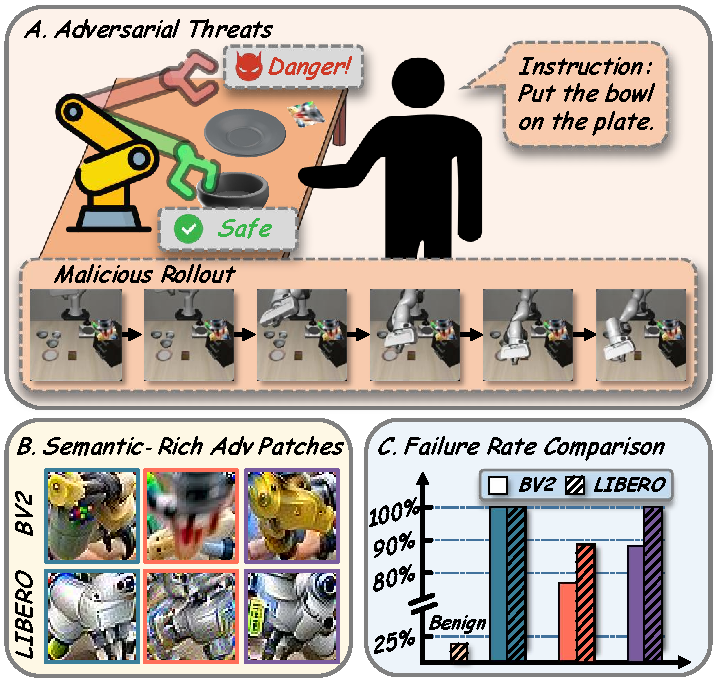
\includegraphics[width=0.47\textwidth]{images/new_fig1.pdf}
    \vspace{-8pt}
    \caption{\textbf{恶意操控诱发的对抗脆弱性}。(A) 机器人任务执行过程中面临的对抗威胁示意图。(B) 本文方法生成的富含语义信息的对抗补丁示例。(C) 不同攻击方案（\textcolor[HTML]{3A7F9A}{\textbf{UADA}}、\textcolor[HTML]{FF6F59}{\textbf{UPA}} 和 \textcolor[HTML]{7A5C9E}{\textbf{TMA}}）下失败率的比较。}
    \label{fig:problems}
    \vspace{-20pt}
\end{figure}

在电影 \textit{Finch} 中，后末日未来背景下的智能机器人围绕复杂主题展开行动，凸显了其与人类主人交互时安全性的重要性。随着大视觉语言模型（Large Vision Language Models, LVLMs）~\cite{wang2024mmpt, xu2024vision}的兴起，这种曾经偏向科幻的设想正变得越来越现实；这类模型能够无缝理解视觉与语言语境。视觉-语言-动作（Vision-Language-Action, VLA）模型~\cite{wang2024towards, ding2025quar, kim24openvla, wen2024tinyvla}则是这一潜力的重要体现，它将 LVLMs 集成到机器人系统中，通过端到端学习同时覆盖高层轨迹规划与底层机器人动作控制。尽管 VLA 模型朝着通用机器人智能迈出了有前景的一步，但它们也引入了大量尚未被充分探索的潜在脆弱性。基于这一认识，本文率先揭示了系统研究基于 VLA 的机器人系统新攻击面的紧迫性。

为了更深入地理解这些脆弱性，我们分析了基于 VLA 的模型与一般机器人操作，并总结出两项对设计有效对抗攻击至关重要的关键特征。首先，为机器人系统设计攻击目标时，必须考虑机器人运动所固有的物理动力学与约束。在这一场景下，传统对抗攻击往往难以导致目标动作发生显著偏移，因为它们忽略了这些约束。其次，VLA 模型生成的控制信号本质上是一个由 \textit{K 类}预测构成的时间序列（见 \S\ref{preliminary}），因此必须设计能够利用序列时间依赖性的攻击，才能对机器人行为造成实质性扰动。如何同时在数字仿真与真实环境中实现有效攻击，仍然关键且具有挑战性。

为了解决这些挑战，我们一方面设计专门化的攻击目标，另一方面提出有效的攻击方法，从而进一步加剧基于 VLA 系统所面临的对抗威胁。具体而言，我们提出了\textbf{动作差异目标}（Action Discrepancy Objective），旨在最大化基于 VLA 的机器人系统中的动作偏差。该策略确保机器人在每个决策点的行为都可能偏离最优轨迹。此外，我们提出了\textbf{几何感知目标}（Geometry-Aware Objective），考虑机器人在三维空间中的运动特性，其对应三个自由度。通过优化对抗方向与真实方向之间的余弦相似度，我们诱导机器人的运动方向偏离原始路径，从而提高任务失败的概率。为实现这些攻击目标，我们进一步设计了针对基于 VLA 机器人系统的简洁而有效的\textbf{基于补丁的攻击}（Patch-Based Attacks）。这一方法使得攻击能够在数字与物理环境中同时生效，揭示出基于 VLA 系统中的显著脆弱性。

综上，这些创新带来了如下重要贡献：\textbf{\ding{182}} 本文首次对基于 VLA 的机器人系统中的脆弱性进行了系统而全面的分析。VLA 是一种利用生成式基础模型训练通用机器人策略的新范式。我们揭示了严重的对抗攻击威胁，强调了在真实世界部署前提升其鲁棒性的迫切需求；\textbf{\ding{183}} 据我们所知，本文首次为强大的 VLA 模型定义了专门的攻击目标，并对其采用了直接的对抗补丁攻击（见 \S\ref{sec:method}）。这为研究社区探索类似并行生成式基础模型中的系统性失效提供了有价值的启示；\textbf{\ding{184}} 我们在模拟环境与真实环境中的四类不同机器人任务上对方法进行了严格评估，分别观察到任务失败率最高提升至 100\% 和 43\%。这充分表明了本文攻击策略的有效性（见 \S\ref{subsec:main_results}）。

\begin{figure}[!t]
    \centering
    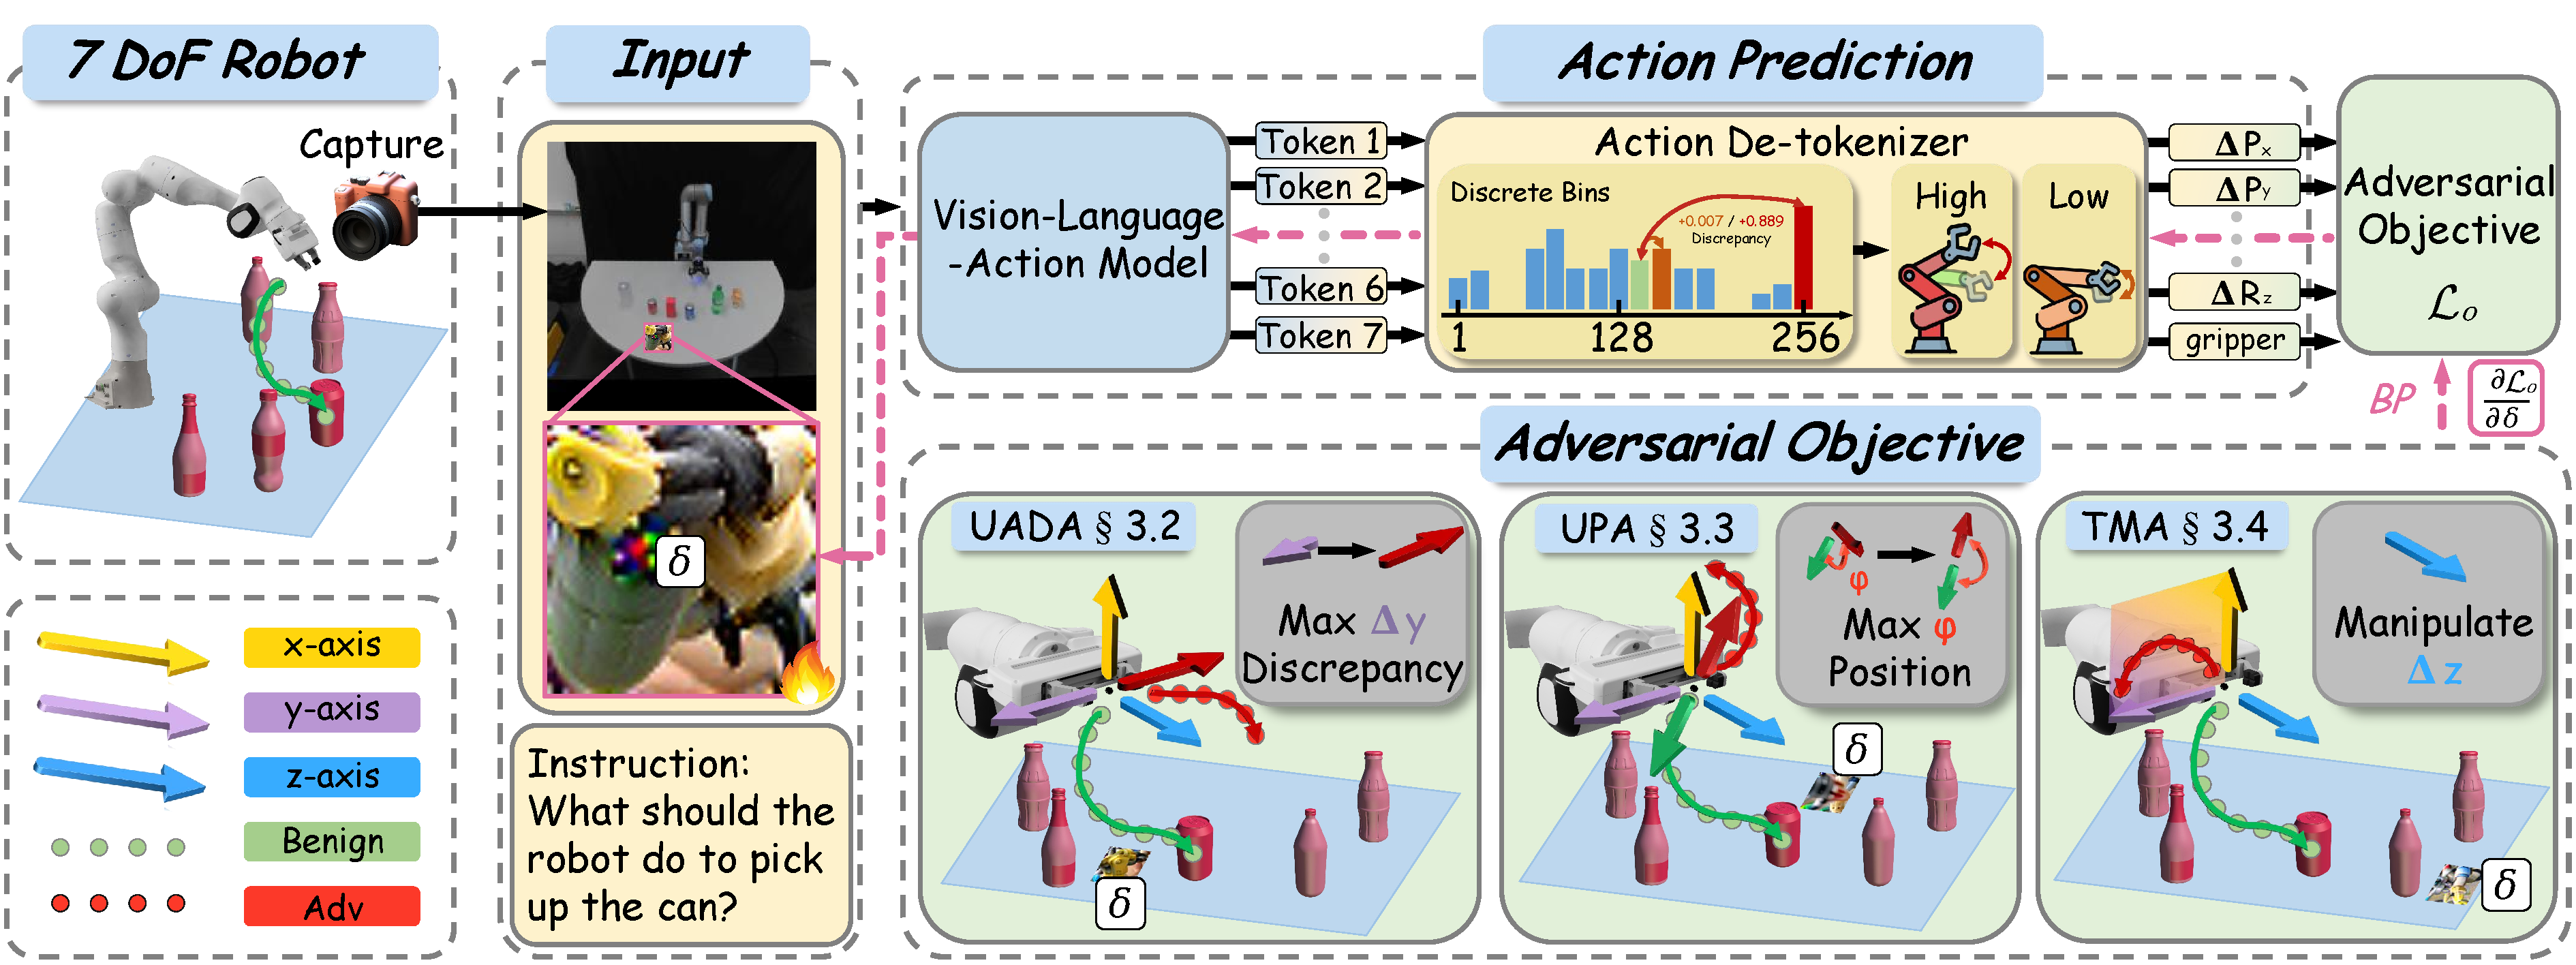
\includegraphics[width=0.95\linewidth]{images/mainfig3.pdf}
    \vspace{-0.8em}
    \caption{\textbf{总体对抗框架}。机器人首先捕获输入图像，经视觉语言模型处理后生成表示动作的 token，再通过动作去标记器进行离散 bin 预测。模型利用不同差异性与几何性对抗目标进行优化（即，UADA、UPA、TMA）。前向传播以黑色表示，反向传播以\textcolor[HTML]{E26C9F}{粉色}突出显示。这些目标旨在最大化误差并最小化任务性能，同时强调三维空间操控，并聚焦于在任务执行过程中生成对抗扰动 $\delta$，例如在拾取易拉罐时。}
    \label{fig:main}
    \vspace{-1.6em}
\end{figure}
